\chapter{Discussion}\label{ch:discussion}

The Results reveal that the onset of hydrogen exsolution from a sub-Neptune magma ocean
cannot be read from equilibrium miscibility data alone. The published mixing model predicts
a metastable window of several hundred kelvin, but the same source data, fitted with the
same or slightly more flexible forms, favour windows two to ten times shorter. In this
chapter, we interpret the physical mechanisms behind these results and discuss how they
bear on the evolution and observable properties of sub-Neptune exoplanets.

\section{Why Equilibrium Data Cannot Fix the Spinodal}\label{sec:why}

The binodal and the spinodal probe different parts of the free energy. The binodal follows
from the common tangent, so it depends only on the free energy at the two coexisting
compositions and on the line between them. The spinodal depends on the local curvature of
the homogeneous free energy between those compositions, where a phase-separated simulation
never samples the homogeneous state. The perturbation of Section~\ref{sec:identifiability}
makes this explicit: it changes the curvature inside the gap and leaves every equilibrium
observable unchanged.

Fitting a smooth model with few parameters ties the curvature inside the gap to the free
energy outside it. The spinodal is then exactly as well constrained as these parameters. For
the baseline parcel three of them matter together: the asymmetry $B/A$, which sets the critical
composition, the excess entropy, set by $\tau$, and the strength of the interaction. The source
data pull them in different directions. Without the homogeneous data, the fit returns to the
published asymmetry ($B/A = \BAMOnePhaseComp{}$), but with a larger excess entropy than the
homogeneous simulations allow. The homogeneous enthalpies, which are almost symmetric about
$x \approx 0.54$, favour a weak asymmetry ($B/A = \BAMOnePhaseHom{}$). The published fit
combines the strong asymmetry with moderate interaction parameters. None of our refits
reproduces this combination, and none has a median window above \IntRangeHi{}\,K. A weaker asymmetry moves the critical composition toward the
baseline parcel and shortens its window. A second tension
concerns the critical curve: its slope, set by the excess volume in all our model classes,
cannot follow both the near-critical runs and the homogeneous volumes
(Section~\ref{sec:recalibrated}).

Close to the critical point, binodal and spinodal are linked more tightly. In mean-field
theory, to leading order, the spinodal lies three times as far below $T_C$ as the binodal at
the same distance from $x_C$ \cite{debenedetti1996}. Near-critical data
therefore constrain the spinodal of near-critical parcels, but not of a parcel at
$x = 0.435$ that lies far from $x_C$. The runs that are most informative about the curvature
are also the runs whose compositions are least certain (Section~\ref{sec:audit}).

\section{Implications for Hydrogen Release and Atmospheric Composition}\label{sec:implications}

Evolution models with hydrogen--silicate miscibility release hydrogen into the envelope as the
binodal moves through the interior \cite{rogers2025,rogers2026,tejada2026}. They assume that
separation starts at the binodal. Our results bound the possible lag. For a parcel with
3\,wt\% local hydrogen at 2\,GPa, nucleation-limited release could lag the binodal by
\IntRangeLo{} to \pubIntTwo{}\,K in temperature, depending on which description of the source
data is adopted. Over this interval, equilibrium would already have moved up to \pubFhTwo{}\%
of the parcel's hydrogen into a separate H-rich phase.

A lag in temperature becomes a lag in time through the cooling rate of the planet at that
stage, which we do not compute. If it is long, it postpones the inflation of the envelope by
exsolved hydrogen and makes the release more abrupt once the spinodal is reached. In our
thesis, the atmospheric hydrogen budget controlled the mean molecular weight $\mu_{\rm atm}$
and the carbon speciation through the methanation equilibrium
CO$_2$ + 4H$_2$ $\rightleftharpoons$ CH$_4$ + 2H$_2$O \cite{laga2025}. A delayed, abrupt
supply of hydrogen would temporarily lower $\mu_{\rm atm}$, shift carbon toward CH$_4$, and
could change the silane--methane competition proposed as a magma-ocean diagnostic
\cite{hakim2026}. These effects remain conditional on the transport of hydrogen from the
interior to the observable atmosphere, which neither this work nor the equilibrium models
resolve. In an earlier sensitivity experiment with the 2025 mixing model (repository
directory \texttt{research/spinodal\_study}), the atmospheric signal of demixing depended
strongly on the assumed transfer of material and on condensation.

Whether the delayed limit applies at all depends on nucleation. Interfaces lower or remove
the nucleation barrier: the magma-atmosphere boundary itself, crystals in a cooling magma
ocean and droplets of an earlier-separated phase can all act as nucleation sites. Deep in a
supercritical interior without such interfaces, separation would instead require homogeneous
nucleation. The metastable window is therefore an upper bound on the lag, and the equilibrium
binodal a lower bound.

\section{A Decisive Simulation Campaign}\label{sec:design}

The posteriors identify which simulations would settle the question. A screen over candidate
measurements uses the posterior samples of all four model classes with equal weight
(Figure~\ref{fig:design}). One new homogeneous simulation at $x \approx \designBestX{}$, with the
precision of the existing ED Table~2 entries, would reduce the posterior standard deviation of
the baseline spinodal only from \designSdNow{}\,K to \designSdAfter{}\,K. Most of the remaining
spread comes from the differences between model classes and between data subsets, which one
more homogeneous point does not remove.

\begin{figure*}[t]
\centering
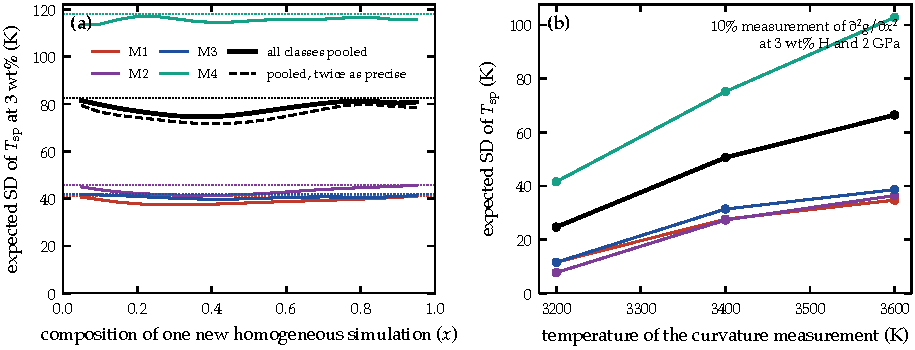
\includegraphics[width=\textwidth]{fig4_1_design}
\thesiscaption{Simulations that would constrain the spinodal.}{Expected posterior standard
deviation of the spinodal temperature of a 3\,wt\% parcel at 2\,GPa after (a) one new
homogeneous simulation of excess enthalpy, entropy and volume at composition $x$, for each
model class (thin lines) and all classes pooled (thick line; dotted lines: current values),
and (b) a measurement of the composition curvature $\partial^2 g/\partial x^2$ at the baseline
composition with 10\% precision, at three temperatures. Linear-Gaussian screen of the
recalibration samples.}
\label{fig:design}
\end{figure*}

A direct measurement of the curvature is more powerful. At 2\,GPa and \curvT{}\,K, a 10\%
measurement of $\partial^2 g/\partial x^2$ would reduce the standard deviation to
\curvSdPooled{}\,K. At this temperature \curvFracStable{}\% of the posterior samples leave the
baseline parcel locally stable: \curvFracMeta{}\% metastable and \curvFracOnePhase{}\% still one
phase. The curvature is accessible without a free-energy model, from the
long-wavelength limit of the Bhatia--Thornton concentration--concentration structure factor,
$S_{cc}(0) = RT/(\partial^2 g/\partial x^2)$ per mole of mixing units
\cite{bhatia1970,kirkwood1951}. Homogeneous DFT-MD simulations of the metastable parcel, in
cells large enough to sample composition fluctuations over several nanometres, could measure
it. Simulations below $T_C$ would also test the assumption of temperature-independent excess
enthalpy and entropy, which all four model classes share.

Even a measured spinodal fixes only the limit of the delay. Its actual length requires the
interfacial tension and the mobility of the mixture. The interface fluctuations in the
existing coexistence simulations could constrain the tension, because their magnitude is
related to it \cite{gilmore2026}. Together
they give nucleation rates through classical nucleation theory \cite{kashchiev2000}, which an
evolution model can then use in place of the two limiting cases studied here.
